\documentclass{ximera}

\title{Review of functions}

\begin{document}
\begin{abstract}
This prelecture is to prepare you for our lecture on functions.
\end{abstract}
\maketitle

In Calculus, we are studying how the output of functions change as the
inputs change. This places functions as the fundamental objects we are
studying in Calculus. If you want a refresher on what functions are,
check this\link{http://en.wikipedia.org/wiki/Function_(mathematics)}
out.


\begin{question}
Which of the following are plots of $y$ as a function of $x$ on the
interval shown?
\begin{solution}
  \begin{multiple-choice}
    \choice[correct]{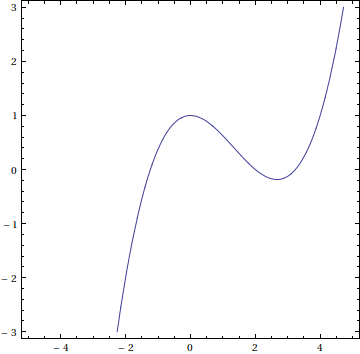
\includegraphics{fxn2a.png}}
    \choice{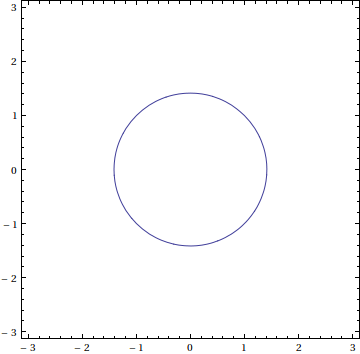
\includegraphics{nonFxn1a.png}}
    \choice{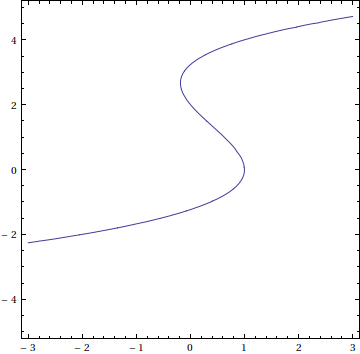
\includegraphics{nonFxn3a.png}}
  \end{multiple-choice}  
\end{solution}
\end{question}

\begin{question}
Which of the following functions are one-to-one on the interval shown?

PICTURES WILL BE IN THE ANSWER

\end{question}

\begin{question}
Why do we care if a function is one-to-one? Select all that are
correct.

CHOICES:

When is a function is one-to-one on an interval, it is invertible on
that interval

\end{question}

\begin{question}
Why is it ``impossible'' to compute $\ln(0)$?
\end{question}

What other questions do you have related to these topics?

\begin{solution}
\begin{freeResponse}
Answers will vary.
\end{freeResponse}
\end{solution}
\end{question}




\end{document}
